\documentclass[12pt,a4paper]{article}

% Margins.
\setlength{\oddsidemargin}{0in}
\setlength{\evensidemargin}{0in}
\setlength{\headheight}{12pt}
\setlength{\headsep}{0pt}
\setlength{\topmargin}{-60pt}
\setlength{\textwidth}{6.5in}
\setlength{\textheight}{10.75in}

\usepackage{float}
\usepackage{graphicx}
\usepackage{datetime}

%opening
\title{\vspace{-1cm}Programming for Engineers I\\Lab 03\\Loops - I}
% '\and' creates even spacing.
\author{Attique Dawood}
\date{February 21, 2013\\[0.2cm] Last Modified: \today, \currenttime}
\begin{document}

\maketitle

\section{Loops (Repetition Statements)}
We have to calculate the sum of first 10 whole numbers i.e. add the numbers from 1 to 10. Following statement may be one way to do it.
\begin{verbatim}
cout << "Sum of first 10 numbers is = " << 1+2+3+4+5+6+7+8+9+10 << endl;
\end{verbatim}
This method is perfectly fine as the syntax is right. The answer is also correct. This procedure can also be adopted while calculating the sum of numbers from 1 to 100. We can write the above statement adding all the digits from 1 to 100. But this method will not be suitable for computing the sum of numbers from 1 to 1000. The addition of a very big number of digits will result in a very ugly and boring statement. 

\section{While Loop}
While means, \emph{do it until the condition is true}. Use of while construct can be helpful in repeating, a set of instructions under some condition. We can also use curly braces with while just like we used with if. If we omit to use the braces with while construct, then only one statement after while will be repeatedly executed. For good programming practices, always use braces with while irrespective of the number of statements in while block. The code will also be indented inside the while block as Indentation makes the code easy to understand. 
The syntax of while construct is as under:
\begin{verbatim}
while ( Logical Expression )
{
    statement1;
    statement2;
    ...
}
\end{verbatim}
The logical expression contains a logical or relational operator. While this logical expression is true, the statements will be executed repeatedly. When this logical expression becomes false, the statements within the while block, will not be executed. Rather the next statement in the program after while block, will be executed. 
% Flow Chart here
\begin{figure}[H]
\centering
\label{While-Loop-Flow-Diagram}
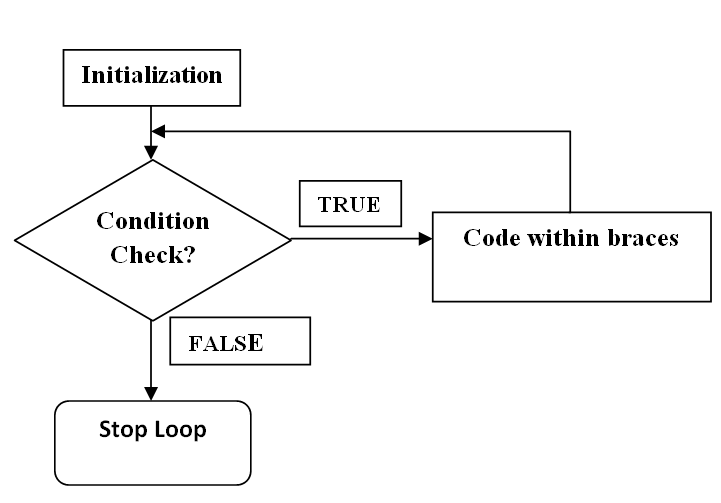
\includegraphics[width=0.8\textwidth]{FlowDiagramWhileLoop.png}
\caption{Flow diagram of while loop}
\end{figure}
\section{Exercise}
% One or more empty lines between text will start a new paragraph.
% '\\' is for next line without starting a paragraph. Paragraph starts with a tab.
\textbf{Question No. 1:} Print the squares of numbers from 1-10\\
\noindent\textbf{Question No. 2:} Write a program that inputs two integers from the user in a loop, takes their difference continues if the difference is a positive number otherwise exits the program. The program keeps on running till the user wishes to quit. 
The syntax of while should be like:
\begin{verbatim}
char c=`N';
while (c!=`Y')
{

}
\end{verbatim}
\noindent\textbf{Question No. 3:} Write a program to print right triangle using loop (Take Height from the user).
\begin{verbatim}
*
**
***
****
*****
\end{verbatim}
\noindent\textbf{Question No. 4:} Write a C++ code to print out all Armstrong numbers from 100 to 999. A number is called Armstrong number if sum of cubes of each digit of the number is equal to the number itself. For example $153=(1^3+5^3+3^3)$.
\noindent\textbf{Question No. 5:} Write a program to print the following shapes using for Loop (Take Height from the user). 
\begin{verbatim}
*           	*****               *       	 *****
**          	****               **       	  ****
***         	***               ***       	   ***
****        	**               ****       	    **
*****       	*               *****       	     *
\end{verbatim}
\end{document}
